% Enable warnings about problematic code
\RequirePackage[l2tabu, orthodox]{nag}

\documentclass{scrartcl}



\author{%
  Sebastian Blei \\ \normalsize{211100448} \\{\normalsize sblei@uni-koblenz.de} \and
  Andrea Mildes \\ \normalsize{212100201} \\{\normalsize mildes@uni-koblenz.de}
}

\title{Assignment 2 \\ hotel}
\date{}

\usepackage{varwidth}
\usepackage{graphicx}

% ==============================================================================
% Document

\begin{document}

\maketitle


% ------------------------------------------------------------------------------

\section{IP Packet (5 Points)}

Consider the IPv4 packet that is received as:\\ \\
\texttt{4500 062A 42A1 8001 4210 XXXX C0A8 0001 C0A8 0003}\\ \\ 
Consider \texttt{XXXX} to be the check sum field that needs to be sent with the packet.\\
Please provide a step-by-step process for calculating the "Check Sum".\\ \\ 
\textbf{\underline{Answer:}}\\
\\
1. Step: calculate the sum of each 16bit value except the checksum\\
4500 + 062A + 42A1 + 8001 + 4210 + C0A8 + 0001 + C0A8 + 0003 = \textbf{2D130}\\
\\
2. Step: Convert 2D130 to binary\\
(2D130)$_{16}$ = (0010 1101 0001 0011 0000)$_{2}$\\
\\
3. Step: Add the carry (first 4 bits) to the rest of the value\\
0010 + 1101 0001 0011 0000 = 1101 0001 0011 0010\\
No new carry has been generated, if it was, we had to add it as well.\\
\\
4. Step: flip 1 to 0 and 0 to 1\\
1101 0001 0011 0010 $\rightarrow$ 0010 1110 1100 1101\\
\\
5. Step: Convert to hexadecimal\\
(0010 1110 1100 1101)$_{2}$ = (2ECD)$_{16}$\\
\\
Thus, our checksum is 2ECD and we receive the package\\
4500 062A 42A1 8001 4210 2ECD C0A8 0001 C0A8 0003


% ------------------------------------------------------------------------------

\section{Routing Algorithm (10 Points)}
You have seen how routing tables can be used to see how the packets are transferred across different networks. Using the routing tables below of Router 1, 2 and 3:
\begin{enumerate}
	\item Draw the network \texttt{[6 points]}
	\item Find the shortest path of sending information from 67.68.2.10 network to 25.30.3.13 network \texttt{[4 points]}
\end{enumerate}

\textbf{\underline{Answer:}}\\
\\
1.)\\
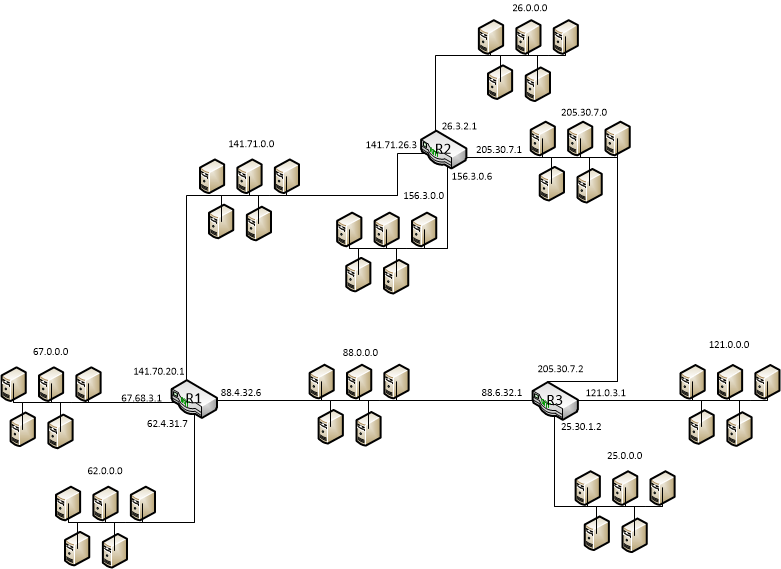
\includegraphics[width=1\textwidth]{21.png}
2.)\\
\\
The hosts sends its information to the Router R1. The Router sends the information through the 88.0.0.0 network to the Router R3. R3 then sends the information to the 25.0.0.0 network, where the receiving host 25.30.3.13 is at.\\
% ------------------------------------------------------------------------------


\section{Sliding Window Protocol (10 Points)}

Let us consider you have 2 Wide Area Networks. One with a bandwidth of 10 Mbps (Delay of 20 ms) and the other with 1 Mbps (Delay of 30 ms) . If a packet is considered to be of size 10kb. Calculate the window size of number of packets necessary for Sliding Window Protocol. [\texttt{5 points}]\\ \\
Since you now understand the concept of Window Size for Sliding Window Protocol and how to calculate it, consider a window size of 3 packets and you have 7 packets to send. Draw the process of \texttt{Selective Repeat Sliding Window Protocol} where in the 3rd packet from the sender is lost while transmission. Show diagrammatically how the system reacts when a packet is not received and how it recuperates from that scenario. [\texttt{5 points}] \\




% ------------------------------------------------------------------------------

\section{TCP Client Server (10 Points)}

Use the information from the socket documentation and create: [\texttt{4 points}]
\begin{enumerate}
\item a simple TCP Server that listens to a
\item Client
\end{enumerate}
Given below are the following points that your client and server must perform: [\texttt{6 points}]
\begin{enumerate}
\item The \emph{Client} side asks the user to input their name, age \& \emph{matrikelnummer} which is then sent to the server all together.
\item Develop a protocol for sending these three information and subsequently receiving each of the information in three different lines as mentioned in the below format. Provide reasons for the protocol you implemented. 
\item Format the output in a readable format as:\texttt{\\ Name: Korok Sengupta; \\ Age: 29; \\ Matrikelnummer: 21223ert56}
\end{enumerate}

Provide a snapshot of the results along with the code. \\


\end{document}
